\begin{center}
  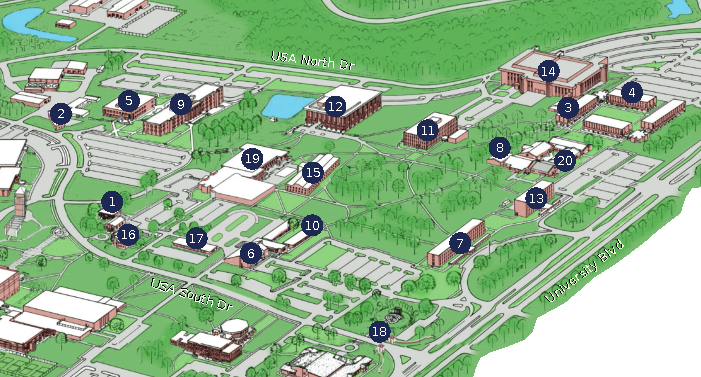
\includegraphics[width=0.9\linewidth]{assets/south-map}
\end{center}

\begin{multicols}{2}
  \begin{enumerate}
    \item Alumni Hall (Codes 000-049) %MP2 30.694363,-88.179506
    \item Archaeology Museum (Codes 050-099)
    \item Central Services Admin Building (Codes 100-149) % 30.69875, -88.17618
    \item Charles M. Baugh Biomedical Library (Codes 150-199) % CP2 30.698756,-88.175708
    \item Chemistry Building (Codes 200-249) % CP3 30.696934,-88.181128
    \item Computer Services Center (Codes 250-299)
    \item F.P. Whiddon Administration Building (Codes 300-349) % MP4 30.6954, -88.17492
    \item Glass Arts Building (Codes 350-399) % 30.69708, -88.17642
    \item Humanities Building (Codes 400-449) % CP4 30.696975,-88.180477
    \item Innovation in Learning Center (Codes 450-499)
    \item Life Sciences Building (Codes 500-549)
    \item Marx Library (Codes 550-599) %MP3 30.697147,-88.178782
    \item Mathematical Sciences and Physics Building (Codes 600-649)
    \item Medical Sciences Building (Codes 650-699)
    \item Meisler Hall (Codes 700-749) % 30.69595, -88.17747
    \item Mobile Townhouse (Codes 750-799)
    \item Student Health Center (Codes 800-849) %CP1 30.694061,-88.178082
    \item Tholos of Delphi Replica (Codes 850-899)
    \item USA Student Center (Codes 900-949)
    \item Visual Arts Complex (Codes 950-999) % MP1 30.697469,-88.175504
  \end{enumerate}
\end{multicols}

To enter a Start Code that unlocks a Main Puzzle or Cryptic Puzzle,
your device's GPS must detect that you are near the front door of 
the location corresponding to the code. 
For example, to enter the Start Code \texttt{123}, you
will need to visit Central Services Admin Building, since
\(100\leq 123\leq 149\).

Players will not need to cross USA South Dr, USA North Dr, or University Blvd.
